%%\documentclass{tufte-book}

\documentclass[bahasa]{tufte-book}
\usepackage[
    type={CC},
    modifier={by-nc-sa},
    version={3.0},
]{doclicense}
\usepackage[lastexercise]{exercise}
\usepackage{xcolor}
\usepackage{mdframed}
\usepackage{amsmath}


\title{Keamanan Informasi}
\author{Budi Rahardjo}

\usepackage{graphicx} % Needed to insert images into the document
\graphicspath{{graphics/}} % Sets the default location of pictures
\setkeys{Gin}{width=\linewidth,totalheight=\textheight,keepaspectratio} % 

\usepackage{makeidx}
\makeindex

\begin{document}


%%\frontmatter
%\fbox{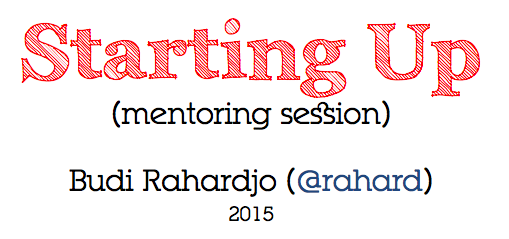
\includegraphics[width=1.0\linewidth]{graphics/BR-starting-up.png}}
%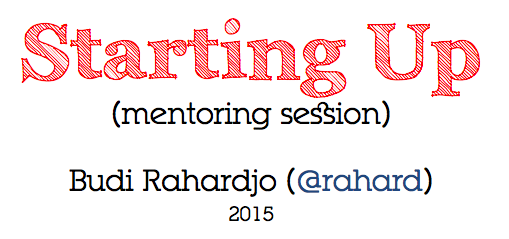
\includegraphics[width=1.0\linewidth]{graphics/BR-starting-up.png}

\maketitle

\tableofcontents

\chapter{Pengantar}

Buku ini muncul karena kebutuhan buku teks untuk kuliah
keamanan informasi ({\em information security}).
Jenis buku seperti ini agak langka.
Bahkan dahulu ilmu yang terkait dengan keamanan - misalnya kriptografi -
dianggap tidak boleh diajarkan sehingga referensi untuk hal itu
sangat langka.
Buku yang pertama kali terbit mengenai kriptografi adalah
``Codebreakers'' karangan David Kahn~\cite{davidkahn},
yang diterbitkan tahun 1969.
Sejak saat ini, ilmu tentang keamanan (security) mulai terbuka untuk umum.

Buku teks berbeda dengan buku {\em how to} yang banyak beredar
di toko buku. Buku tersebut biasanya hanya menjelaskan bagaimana
menggunakan sebuah program tertentu, atau melakukan hal tertentu.
Sementara itu buku teks digunakan untuk memberikan landasan teori
sehingga pemahaman tidak bergantung kepada {\em tools} tertentu saja.
Meskipun demikian, penggunaan {\em tools} sebagai contoh akan
juga disampaikan dalam buku ini.
Semoga dengan demikian, buku ini dapat bertahan lebih lama.
(Meskipun saya agak ragu setelah melihat pesatnya perkembangan
teknologi informasi.)

Urutan pembahasan juga membuat saya merenung cukup panjang.
Ada beberapa hal yang disinggung di depan, tetapi pembahasan teorinya
di belakang. Sementara itu kalau teorinya diletakkan di depan,
maka siswa akan bosan karena terlalu banyak teori.
Seharusnya memang buku ini dipaketkan dengan materi presentasi
(slide) yang saya gunakan untuk mengajar. 
Yang itu belum saya benahi. Masih menunggu waktu.

Sebelumnya saya pernah membuat buku yang sejenis, tetapi kode sumber
dari buku tersebut sudah hilang.
Maklum, saya membuatnya di tahun 1990-an dengan menggunakan program
FrameMaker, yang sudah tidak saya miliki lagi.
Sekarang saya buat dari awal dengan menggunakan \LaTeX \ agar
lebih bisa bebas.

Ada yang mengatakan bahwa {\em security} itu seperti pisau yang bermata dua.
Dia dapat digunakan untuk kebaikan atau kejahatan, tergantung kepada
penggunanya. Saya berharap agar ilmu yang diperoleh dari membaca buku ini dapat
digunakan untuk kebaikan, bukan kejahatan. Saat ini masih dibutuhkan banyak
tenaga kerja yang menguasai security (security professionals). Sayang sekali
kalau lowongan ini tidak dapat dipenuhi dan malah banyak yang memilih untuk
menjadi perusak.

Bagi Anda yang mengajarkan kuliah {\em security} dan ingin menggunakan
buku ini sebagai buku teks, silahkan digunakan.
Bagi para mahasiswa dan peneliti yang membutuhkan referensi untuk
makalah Anda, semoga buku ini dapat membantu.
Lebih baik lagi apabila Anda dapat menemukan guru yang dapat membantu Anda
dalam memahami isi buku ini.
Selain buku ini, saya juga menulis buku lain yang dapat diunduh juga:
``Keamanan Perangkat Lunak''~\cite{BRsecuresoftware}.
Yang ini saya gunakan untuk kuliah saya yang lainnya.

Dikarenakan buku ini masih dalam pengembangan, maka ada banyak bagian yang
masih kosong atau meloncat. Mohon dimaafkan. Dalam penulisan selanjutnya,
bagian-bagian tersebut akan diisi dan dilengkapi. Mohon masukkan jika hal ini
terjadi.

Selamat menikmati versi 0.2 dari buku ini. Semoga bermanfaat.
\vspace{5 mm}

Bandung, 2017


Budi Rahardjo, peneliti\\
twitter: @rahard\\
blog: http://rahard.wordpress.com\\
web: http://budi.rahardjo.id

\vspace{5 mm}
Penulisan referensi:\\
Budi Rahardjo, {\em ``Keamanan Informasi''}, PT Insan Infonesia, 2017.

\doclicenseThis

\chapter{Pendahuluan}
Selalu ada aspek negatif dari sebuah pemanfaatan teknologi.
Teknologi informasi tidak lepas dari masalah ini.
Ada banyak manfaat dari teknologi informasi.
Sayangnya salah satu aspek negatifnya adalah masalah keamanan
({\em security}).

Banyak tulisan dan buku yang mengajarkan cara merusak sebuah
sistem informasi. Sementara itu buku yang mengajarkan cara
pengamanannya agak minim. Demikian pula, ilmu untuk mengamankan
sistem berbasis teknologi informasi juga harus lebih banyak
diajarkan.

%%%
\section{Keamanan Informasi}
Ketika kita berbicara tentang {\em security}, yang muncul dalam
benak kebanyakan orang adalah {\em network security}, keamanan jaringan.
Padahal sesungguhnya yang ingin kita amankan adalah \textbf{informasi}.
Bahwa informasi tersebut dikirimkan melalui jaringan adalah benar,
tetapi tetap yang ingin kita amankan adalah informasinya.
Nanti akan kita bahas lebih lanjut mengapa demikian.
Maka judul dari buku ini adalah ``Keamanan Informasi''.

%%%
\section{Beberapa Contoh Kasus}
Untuk menunjukkan betapa banyaknya masalah keamanan informasi,
berikut ini ada beberapa contoh kasus-kasus.
Contoh ini bukanlah daftar yang komplit, melainkan hanya sampel
dari kondisi yang ada. Bahkan, kemungkinan kondisi yang ada
lebih parah daripada contoh-contoh ini.

Beberapa contoh kasus di luar negeri (diurutkan berdasarkan
tahun kejadiannya) antara lain dapat dilihat dari daftar berikut.

\begin{enumerate}
\item 2006-2008. Tahun-tahun ini ditandai dengan mulai masuknya
   aspek manajemen ke dalam bidang keamanan informasi.
   Standar ISO (mulai dari 17799 dan kemudian menjadi seri 27000)
   mulai digunakan di berbagai instansi.
   Adanya bencana alam (tsunami, banjir, gempa, dan sejenisnya)
   membuat orang mulai memikirkan keberlangsungannya sistem IT.
   Perangkat IT semakin mengecil dalam ukuran sehingga mulai dibawa
   pengguna ke kantor. Misalnya pengguna membawa sendiri akses
   internet dengan menggunakan handphone 3G.
   Penggunaan kartu sebagai pengganti uang juga mulai populer.
   (Less cash society.)

\item 2013. Virus masih tetap mendominasi masalah.
   Pencurian identitas ({\em identity theft}) mulai marak.
   Cyber war mulai menjadi bagian dari diskusi.
\item 2014. Heartbleed dan Bash Bug.
   (Yang ini lebih mudah dijelaskan dengan menggunakan gambar.
   Sayangnya saya tidak memiliki hak untuk memasukkan gambar tersebut
   ke dalam buku ini. Di kesempatan berikutnya akan saya usahakan
   memberi penjelasan dengan kata-kata dulu.)
\item 2014. Bursa Singapura terganggu karena masalah software.
   Perdagangan saham sempat terhenti.
\item 2016.
   Sebuah firma hukum di Panama bernama Mossack Fonseca (MF)
   mengalami kebocoran data.
   Data yang bocor berupa tabungan / investasi orang-orang terkenal
   dari beberapa negara (termasuk Indonesia).
   Kasus ini disebut {\em Panama Papers Breach}.
   Kebocoran ini diduga karena {\em Slider plugin} yang digunakan
   oleh situsnya (yang menggunakan Wordpress) sudah kadaluawarsa dan
   memiliki kerentanan. Hasil eksploitasi memperkenankan orang untuk
   mengambil berkas sesukanya.
\item 2016. 
   CCTV digunakan sebagai bagian dari Distributed DoS attack.
   Ini menunjukkan bahwa perangkat yang menjadi bagian dari
   Internet of Things (IoT) dapat menjadi target serangan
   untuk kemudian dijadikan ``anak buah'' (zombie) untuk
   menyerang tempat lain.
   Kode sumber Mirai yang digunakan untuk melakukan penyerangan
   tersedia di internet. Jika kita tidak siap, ini dapat menjadi
   masalah yang berikutnya.
\item 2016.
   Serangan DDoS terhadap berbagai DNS (Domain Name System) servers.
   Serangan menggunakan bantuan {\em botnet}
   sehingga menghabiskan {\em bandiwdth} jaringan dalam orde
   Gbps.
\item 2017.
   Sebuah kampus di Amerika Serika mengalami masalah di jaringan internalnya.
      Ternyata ada banyak paket dari segmen mesin minuman (atau segmen IoT).
      Perangkat IoT ternyata diretas (melalui coba-coba password secara
      brute-force). Kemudian perangkat tersebut menyerang DNS dari kampus.
\item Februari 2017. 
   Layanan cloud dari Amazon.com berhenti berfungsi (down) selama beberapa jam.
      Berbagai perusahaan yang menyediakan layanan untuk publik dan kebetulan
      menggunakan layanan cloud (S3) dari Amazon ikut berhenti. Setelah
      diteliti, penyebabnya adalah salah ketik (typo) dari salah seorang
      operator~\footnote{Catatan dari Amazon dapat dibaca di sini: https://aws.amazon.com/message/41926/}.
   \item Mei 2017. Dunia digemparkan dengan Ransomware WannaCry yang menyerang
      hampir semua versi dari sistem operasi Microsoft Windows. Penyerangan
      memanfaatkan kelemahan dari SMBv1. Sebetulnya dari sisi teknis,
      ransomware ini tidak lebih hebat dari yang lain-lainnya tetapi nampaknya
      wawasan akan keamanan mulai terbangun. (Meskipun ada reaksi yang terlalu
      berlebihan.) Salah satu dokumentasi cara penanganannya dapat dibaca di
      blog~\cite{brwannacry}\footnote{https://rahard.wordpress.com/2017/05/14/
      penanganan-ransomware-wannacry/}.
\item 27 Mei 2017. Sistem komputer dari penerbangan British Airways (BA) gagal
   berfungsi. Akibatnya seluruh penerbangan terkait dengan BA dihentikan.
      Penumpang terkatung-katung. Diberitakan bahwa software tidak berfungsi
      dan kemungkinan penyebabnya adalah masalah {\em power}.
   \item Juni 2017. Kembali terjadi serangan ransomware yang diberi nama Petya.
      (Nama ini diberikan karena pada awalnya diduga kodenya mirip dengan kode
      yang diberi nama Petya, tetapi penelusuran lebih jauh ternyata
      menunjukkan bahwa kodenya berbeda.) Pada dasarnya ransomware ini
      melakukan eksploitasi kelemahan pada SBM v1, seperti pada ransomware
      WannaCry. Diduga eksploit ini juga berasal dari eksploit EtherBlue yang
      dikembangkan oleh NSA. Ransomware Petya ini pertama kali ditemukan di
      Ukraina. Diperkirakan awalnya disebarkan melalui software akunting yang
      harus digunakan oleh perusahaan yang memiliki kontrak dengan pemerintah
      Ukrainia. Itulah sebabnya ada dugaan lain bahwa sebetulnya serangan ini
      ditargetkan untuk menyerang atau mengacaukan Ukraina. Penyebaran
      ransomware ini agak terbatas karena mekanisme penyebarannya melalui
      jaringan lokal, bukan internet meskipun upaya penyebaran melalui 
      {\em pishing} juga ada..
   \item 13 September 2017. Aplikasi chat Telegram down sehingga tidak dapat
      digunakan. Diduga permasalahan disebabkan oleh listrik di data center
      mereka yang berada di Singapura. Ini adalah masalah {\em availability}.
      Padahal permasalahan listrik di data center Singapura seharusnya tidak
      menjadi masalah.
      \begin{figure}[ht]
      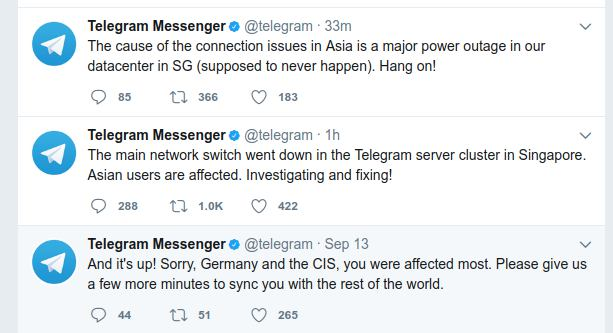
\includegraphics[width=1.0\linewidth]{graphics/telegram-down.jpg}
      \caption{Telegram down}                                                   
      \label{fig:telegram-down}                                                 
      \end{figure}
\end{enumerate}

Selain contoh-contoh di atas, tentunya masih banyak kasus-kasus lain.
Ada yang menganalogikan ini sebagai puncak dari {\em iceberg}.
Di bawah laut lebih banyak lagi masalah yang tidak terlihat.

Beberapa contoh kasus yang terkait dengan Indonesia dapat
dilihat dari daftar berikut.

\begin{enumerate}
\item 1999. Nama domain Timor Timur (.TP) diacak-acak.
   Diduga pelakunya adalah pemerintah Indonesia.
   Investigasi lebih lanjut menunjukkan bahwa ini tidak dilakukan
   oleh pemerintah Indonesia tetapi oleh seseorang (atau sekelompok)
   yang berada di Amerika Serikat.
\item 2011. Perusahaan Research in Motion (RIM) yang memproduksi
   {\em Blackberry} dipaksa untuk memiliki server di Indonesia.
   Alasan utama adalah agar dapat dilakukan {\em lawful interception},
   yaitu penyadapan secara legal untuk kasus-kasus tertentu.
   Pihak RIM keberatan. Tidak ada server RIM di Indonesia.
\item 2015. Serangan man-in-the-browser (MITB) dilakukan terhadap
   berbagai layanan internet banking di Indonesia sehingga mengakibatkan
   hilangnya uang nasabah\footnote{http://regional.kompas.com/read/
   2015/08/11/12185971/
   Kronologi. Hilangnya. Uang. Nasabah. Bank. Mandiri.
   Versi. Korban}
\item 2016. Aplikasi Pokemon Go mulai muncul dan ramai digunakan.
   Aplikasi ini menggunakan lokasi pengguna sebagai bagian dari
   permainannya, yaitu untuk menampilkan monster Pokemon sesuai
   dengan lokasi.
   Selain itu, foto dari lingkungan sekitarnya dapat juga kita ambil
   dan kita bagikan (share) dengan orang lain melalui media sosial.
   Aplikasi ini dilarang digunakan di lingkungan milter dan
   pemerintahan karena dikhawatirkan dapat membocorkan data rahasia.
   (Sebetulnya ada banyak aplikasi lain yang juga menggunakan data
   lokasi seperti {\em Waze} dan {\em Google Maps}, tetapi ini tidak
   ``terlihat''. Bahkan lebih berbahaya lagi adalah penggunaan
   layanan email gratisan untuk akun resmi pemerintahan atau instansi
   lain di Indonesia.)
\item 2016.
   Berbagai {\em market place} (seperti Tokopedia, Bukalapak, dll.)
   dan aplikasi handphone (seperti Go-Jek) diserang oleh orang
   yang mencoba melakukan password cracking.
   Asumsinya adalah seseorang akan menggunakan userid (alamat email)
   dan password yang sama untuk situs-situs tersebut.
   Identitas yang bocor di sebuah layanan (web site, application)
   dicoba digunakan di tempat lain. 
\item 2016. Topik pembentukan ``Badan Cyber Nasional (BCN)''
   mulai hangat dibicarakan.
\item 2017. Seorang (beberapa?) mahasiswa di sebuah perguruan tinggi
   di Indonesia meminta bantuan cracker untuk mengubah nilainya di
   sistem informasi kampusnya.
\item Maret 2017. Listrik dari tempat data center dari sebuah ISP mati sehingga
   layanannya terhenti. Beberapa {\em electronic market places} ikut terkena
      imbasnya karena menggunakan layanan ISP tersebut.
\item Agustus 2017. Satelit Telkom 1 mengalami masalah sehingga ribuan ATM
   dari berbagai bank di Indonesia tidak dapat beroperasi. Satelit ini
   memang sudah habis masa operasinya, meskipun diperkirakan masih dapat
   digunakan beberapa tahun lagi. Dipertanyakan kesiapan dari {\em business
   continuity planing} dari layanan ATM bank.
\end{enumerate}

Saat ini semakin banyak lagi masalah keamanan yang ditemui.
Hal ini disebabkan semakin banyak pemanfaatan teknologi informasi dan
jaringan internet.
Selain itu teknik untuk menemukan lubang keamanan juga semakin
canggih sehingga lebih banyak ditemukan kelemahan-kelemahan tersebut.

Sebuah survey yang dilakukan oleh {\em Information Week} di Amerika
Serikat (tahun?) menunjukkan bahwa hanya 22 persen manager yang
menganggap keamanan sistem informasi sebagai hal yang penting.
Bagaimana meyakinkan mereka untuk melakukan investasi di pengamanan?

Rendahnya kesadaran atas masalah keamanan (lack of security awareness)
merupakan salah satu kunci utama munculnya masalah keamanan.
Para praktisi juga masih menjalankan kebiasaan buruk,
seperti misalnya berbagi password admin.

Masalah keamanan informasi yang biasanya berupada data teknis
harus diterjemahkan ke angka finansial agar dapat dimengerti 
oleh pihak pimpinan.
Sebagai contoh, di Inggris ada survey mengenai berapa biaya
yang dikeluarkan perusahaan jika sistem mereka tidak dapat
diakses ({\em down}).



\section{Security Life Cycle}
Banyak orang yang beranggapan bahwa masalah keamanan informasi
dapat dipecahkan dengan membeli produk keamanan,
misalnya firewall, anti-virus, dan seterusnya.
Kemanan informasi sebetulnya berupa sebuah siklus
sebagaimana ditampilkan pada Gambar~\ref{fig:security-life-cycle}.

\begin{figure}[ht]
\fbox{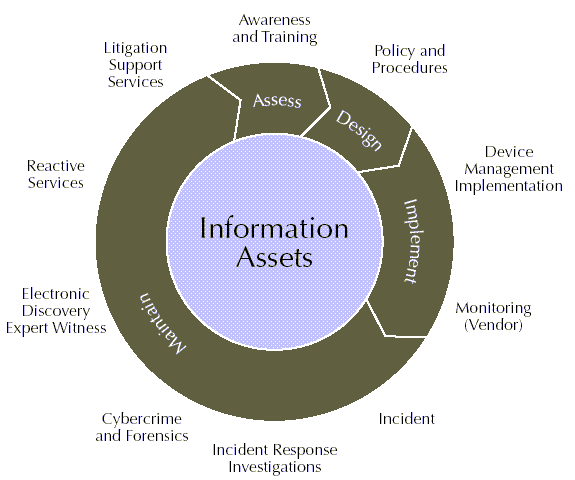
\includegraphics[width=1.0\linewidth]{graphics/security-life-cycle.png}}
\caption{Security Life Cycle}
\label{fig:security-life-cycle}
\end{figure}

Sesuatu yang akan kita amankan disebut dengan ``aset''. Untuk itu, langkah
pertaman dalam pengamanan adalah menentukan aset yang ingin dilindungi. Apa saja
yang dianggap sebagai aset harus ditentukan bersama dengan pemilik dari sistem
(aplikasi, data, dsb.) sebab mereka yang mengetahui mana aset dan mana yang
bukan aset.
Proses ini disebut {\em assesment} dan dapat dilakukan dengan melalui training
atau {\em awareness} terhadap pihak-pihak terkait. Seringkali pemilik aplikasi
memahami mana asetnya tetapi pihak operasional (orang-orang IT yang diberi
tugas untuk mengamankan sistem) tidak tahu.

Setelah mengetahui aset yang ingin diamankan, aset tersebut harus kita beri
harga (value). Pengamanan nantinya akan disesuai dengan dengan nilai dari aset
tersebut. Akan sulit kita melakukan investasi pengamanan yang biasanya lebih
mahal dari nilai asetnya. Sebagai contoh, jika kita memiliki sebuah komputer
yang harganya Rp.~5.000.000,- maka akan sulit untuk menerima biaya pengamanan
yang harganya Rp.~100.000.000,- (lebih mahal). Biaya pengamanan harus lebih
murah daripada nilai asetnya. Jika biaya pengamanan lebih mahal, mungkin lebih
baik membeli barang sejenis saja sebagai duplikat.

Untuk hal-hal yang terkait dengan teknologi informasi, pendaftaran aset-aset
ini tidak mudah karena ada hal-hal yang tidak terlihat secara kasat mata.  Aset
ini dapat kita bagi menjadi tiga (3) jenis; {\em hardware}, {\em software}, dan
data. Mari kita mulai mencoba mendata.

Aset yang berbentuk perangkat keras (hardware) agak ``mudah'' didata karena
terlihat oleh mata, tetapi ada beberapa hal yang membuatnya menjadi susah.
Salah satunya adalah nilai dari aset tersebut. Harga komputer cenderung jatuh
dengan cepat. Berapa depresiasi dari sebuah server?  Contoh-contoh aset
perangkat keras antara lain komputer, router, perangkat jaringan, disk, dan
seterusnya. Apakah notebook termasuk aset atau barang habis? Bagaimana dengan
USB flashdisk? Apakah itu termasuk aset juga?

Beberapa kejadian terkait dengan kesulitan mendata perangkat keras antara lain
tidak diketahuinya pemilik dari perangkat tersebut. Database perangkat keras
sering tidak tersedia. Sebagai contoh, sering kali tidak diketahui harddisk dan
lokasi server yang menggunakan disk tersebut.

Jika pendataan perangkat keras sudah susah, maka pendataan perangkat lunak
lebih susah lagi. Masalahnya, perangkat lunak tidak terlihat secara kasat mata
sehingga pendataannya harus melalui pemilik layanan / pemilik aplikasi. Sebagai
contoh, sebuah layanan online memiliki aplikasi di server web dan juga database
di server database. Aplikasi-aplikasi tersebut berbentuk beberapa perangkat
lunak yang tentunya memiliki harga.

Penentuan harga (nilai) dari perangkat lunak cukup rumit. Untuk aplikasi yang
dibeli, dapat digunakan harga pembelian tersebut. Bagaimana menentukan harga
aplikasi yang dikembangkan sendiri? Ada yang menggunakan jumlah waktu
pengembang (dalam {\em man days}) yang kemudian dikalikan dengan honor (gaji)
orang tersebut. Itulah harga dari aplikasi tersebut. Lantas bagaimana dengan
produk {\em free software} atau (sebagian dari) {\em open source} yang
kebanyakan dapat diperoleh secara gratis? Bagaimana menentukan harga mereka?
Ini masih menjadi pertanyaan. Hal lain yang menyulitkan adalah berapa
depresiasi dari perangkat lunak?

Bagian selanjutnya dari aset teknologi informasi adalah data. Jika pendaftaran
aset hardware dan software sudah sukar, pendaftaran data lebih sukar lagi. Data
apa saja yang dimiliki oleh sistem? Pada umumnya data apa saja yang tersedia
tidak terdaftar. Masing-masing aplikasi hanya memiliki data tersendiri.

Penentuan harga dari data lebih sukar lagi. Sebagai contoh, berapa harga data
transkrip mahasiswa? Bagi mahasiswa, data tersebut sangat berharga sehingga
harus dilindungi. Bagi orang lain, data tersebut mungkin tidak ada nilainya.
Maukah Anda membeli data transkrip mahasiswa ITB seharga Rp.~30.000.000,-~?
Saya yakin tidak ada yang mau. Bagaimana jika Rp.~3.000.000,- saja? Mungkin
masih tidak. Bagaimana jika Rp.~3.000,-~? Mungkin mau. Apakah nilai dari data
transkrip tersebut hanya tiga ribu rupiah? Jika iya, bagaimana nilai
perlindungan yang akan kita berikan?


Setelah mengetahui aset yang akan dilindungi, langkah pertama yang dilakukan
adalah melakukan desain pengamanan. Hal ini dilakukan dengan mengembangkan
kebijakan dan prosedur ({\em policies and procedures}). Banyak yang melupakan
langkah ini dan langsung melakukan implementasi, tetapi tanpa PnP ini akan
sulit. Sebagai contoh, siapa yang boleh melakukan akses kepada data transkrip
tersebut? Ini dituangkan dalam kebijakan. Tanpa kebijakan ini, perangkat
pengamanan yang ada (authorization dan access control) akan sulit diterapkan.
Rules apa yang akan dipakai? Banyak kejadian sistem pengamanan diterapkan
dengan salah karena tidak memiliki desain yang benar.

Desain pengamanan ini kemudian diterapkan secara teknis melalui perangkat
pengamanan ({\em security devices}). Penerapan ini dapat meminta bantuan
vendor. 

Meskipun sudah diterapkan pengamanan, insiden keamanan akan tetap dapat
terjadi. Ketika insiden ini terjadi, maka harus dilakukan investigasi terlebih
dahulu. Apakah insiden yang terjadi tersebut benar-benar insiden ataukah
kejadian biasa saja? Jika memang itu adalah insiden, maka akan diproses lebih
lanjut sesuai dengan kebijakan dan prosedur yang ada.

Ini kemudian menjadi siklus; {\em security life cycle}. Banyak orang yang masih
menganggap {\em security} adalah sebuah produk sehingga mereka lebih fokus
kepada pembelian produk pengamanan tertentu tanpa memperhatikan faktor lain
(misalnya aset mana yang akan dilindungi). Ini seperti mengatasi sakit kepala
dengan menggunakan obat penghilang rasa sakit tanpa perlu mencari tahu apa
sumber permasalahan sesungguhnya.


\section{Keamanan Dari Berbagai Elemen Sistem}
Dahulu, ketika kita berbicara tentang {\em security}, maka yang ada dalam
kepala sebagian besar orang adalah {\em network security} (keamanan jaringan
komputer). Padahal sistem teknologi informasi tidak hanya jaringan saja. Ada
elemen-elemen lain di sistem.

Sebuah sistem berbasis teknologi informasi memiliki beberapa elemen (komponen),
yaitu komputer (host, server, workstation), jaringan (beserta perangkatnya),
dan aplikasi (software, database). Keamanan dari masing-masing elemen tersebut
akan berbeda penanganannya.

\subsection{Computer Security}
{\em Computer security} (keamanan komputer) terkait dengan keamanan komputer,
yang boleh jadi merupakan server, workstation, notebook, dan sejenisnya.
Seringkali ini disebut juga sebagai {\em host security}.

Permasalahan yang muncul pada keamanan komputer terkait dengan sistem operasi
yang digunakan, {\em patch} yang sudah dipasang, konfigurasi yang digunakan,
serta keberadaan aplikasi yang ada. Seringkali sistem operasi yang digunakan
sudah kadaluwarsa dan sudah ditemukan beberapa kerentanan (vulnerability) pada
sistem operasinya.

\subsection{Network Security}
Saat ini sebagian besar sistem terhubung dengan jaringan (apapun jenis
jaringannya). Ada beberapa masalah terkait dengan keamanan jaringan, seperti
misalnya penyadapan data, modifikasi data, dan juga serangan {\em Denial of
Service} terhadap jaringan dengan membanjiri jaringan dengan paket yang sangat
banyak (sangat besar).


\subsection{Application Security}
Boleh jadi komputer (server) yang digunakan sudah aman dan jaringan yang
digunakan sudah aman, tetapi aplikasi (software) yang digunakan memiliki
kerentanan sehingga data dapat diambil (atau diubah) oleh orang yang tidak
berhak. Contoh yang sering terjadi saat ini adalah {\em SQL injection}.

Terkait dengan application security adalah keamanan sistem database.
Ternyata penanganan masalah keamanan database mirip dengan penanganan keamanan
jaringan (bukan aplikasi).

Topik keamanan aplikasi atau software mulai menjadi penting dan ini menjadi
topik buku tersendiri.

\chapter{Prinsip-prinsip Keamanan Informasi}

Ada beberapa prinsip utama dalam keamanan informasi.
Bab ini akan membahas prinsip-prinsip tersebut secara singkat.
Hal-hal yang lebih rinci dan teknis, misalnya bagaimana mengimplementasikan
aspek keamanan CIA, akan dibahas pada bagian terpisah.

\section{Aspek Keamanan}
Ketika kita berbicara tentang keamanan informasi, maka yang kita
bicarakan adalah tiga hal;
{\em confidentiality}, {\em integrity}, dan {\em availability}.
Ketiganya sering disebut dengan istilah \textbf{CIA},
yang merupakan gabungan huruf depan dari kata-kata tersebut.
Selain ketiga hal tersebut, masih ada aspek keamanan lainnya.

\subsection{Confidentiality}
{\em Confidentiality} atau kerahasiaan adalah aspek yang biasa dipahami
tentang keamanan.
Aspek confidentiality menyatakan bahwa data hanya dapat diakses
atau dilihat oleh orang yang berhak.
Biasanya aspek ini yang paling mudah dipahami oleh orang.
Jika terkait dengan data pribadi, aspek ini juga dikenal dengan
istilah {\em Privacy}.

Serangan terhadap aspek confidentiality dapat berupa
penyadapan data (melalui jaringan),
memasang {\em keylogger} untuk menyadap apa-apa yang diketikkan
di keyboard,
dan pencurian fisik mesin / disk yang digunakan untuk menyimpan data.

Perlindungan terhadap aspek {\em confidentiality} dapat dilakukan
dengan menggunakan kriptografi, 
dan membatasi akses (segmentasi jaringan)


\subsection{Integrity}
Aspek {\em integrity} mengatakan bahwa data tidak boleh berubah
tanpa ijin dari yang berhak.
Sebagai contoh, jika kita memiliki sebuah pesan atau data 
transaksi di bawah ini (transfer dari rekening 12345 ke rekening 6789 
dengan nilai transaksi teretentu), 
maka data transaksi tersebut tidak dapat diubah seenaknya.

\begin{verbatim}
TRANSFER 12345 KE 6789 100000
\end{verbatim}

Serangan terhadap aspek {\em integrity} dapat dilakukan oleh
{\em man-in-the-middle}, yaitu menangkap data di tengah jalan
kemudian mengubahnya dan meneruskannya ke tujuan.
Data yang sampai di tujuan (misal aplikasi di web server) tidak tahu
bahwa data sudah diubah di tengah jalan.

Perlindungan untuk aspek {\em integrity} dapat dilakukan dengan
menggunakan {\em message authentication code}.


\subsection{Availability}
Ketergantungan kepada sistem yang berbasis teknologi informasi
menyebabkan sistem (beserta datanya) harus dapat diakses ketika dibutuhkan.
Jika sistem tidak tersedia, {\em not available}, maka dapat terjadi
masalah yang menimbulkan kerugian finansial atau bahkan nyawa.
Itulah sebabnya aspek {\em availability} menjadi bagian dari keamanan.

Serangan terhadap aspek {\em availability} dilakukan dengan tujuan
untuk meniadakan layanan atau membuat layanan menjadi sangat lambat
sehingga sama dengan tidak berfungsi.
Serangannya disebut {\em Denial of Service} (DOS).

Perlindungan terhadap aspek {\em availability} dapat dilakukan
dengan menyediakan redundansi.
Sebagai contoh, jaringan komputer dapat menggunakan layanan dari
dua penyedia jasa yang berbeda.
Jika salah satu penyedia jasa jaringan mendapat serangan (atau rusak),
maka masih ada satu jalur lagi yang dapat digunakan.


%%%
\section{Aspek Keamanan Lainnya}
Selain ketiga aspek utama (CIA), yang sudah dibahas pada bagian sebelumnya,
ada aspek keamanan lainnya. Yang ini sifatnya tambahan, meskipun
kadang menjadi bagian yang cukup signifikan juga.

\subsection{Non-repudiation}
Aspek {\em non-repudiation} atau nir-sangkal digunakan untuk
membuat para pelaku tidak dapat menyangkal telah melakukan sesuatu.
Aspek ini biasanya kental di dalam sistem yang terkait dengan transaksi.
Contoh penggunaannya adalah dalam sistem lelang elektronik.

Implementasi dari aspek ini dapat dilakukan dengan menggunakan
{\em message authentication code} (dengan menggunakan fungsi {\em hash})
dan pencatatan (logging).

\chapter{Kriptografi}
Ada dua cara untuk mengamankan data, yaitu menyembunyikan data atau menyandikan
data. Cara pertama menggunakan steganografi, sementara cara kedua menggunakan
kriptografi. Bab ini akan membahas lebih banyak tentang kriptografi, meskipun
steganografi akan disinggung secara singkat.

Ilmu ini pada awalnya dianggap terlarang untuk diajarkan sehingga tidak ada
bahan bacaan untuk mempelajarinya. Setelah David Kahn membuat bukunya di tahun
1969, maka ilmu pengamanan data ini menjadi lebih terbuka untuk dipelajari.
Saat ini sudah sangat banyak buku yang membahas mengenai hal ini, mulai dari
yang umum~\cite{levycrypto} (tidak teknis) sampai ke yang teknis.


\section{Steganografi}
Steganografi ({\em steganography}) adalah ilmu untuk menyembunyikan pesan
sehingga tidak terlihat dengan mudah. Mekanisme penyembunyian ({\em hide}, {\em
concealment}) dilakukan dengan menggunakan media lain. Sebagai contoh, kita
dapat menyembunyikan pesan dalam gambar ({\em image}, foto), audio, atau video.
Dalam sejarahnya, penyembunyian pesan dapat dilakukan dengan menggunakan meja
yang dilapisi lilin (jaman perang antara Yunani dan Persia).

Saat ini steganografi digunakan sebagai bagian dari {\em Digital Rights
Management} (DRM), misalnya dengan menyisipkan informasi mengenai HaKI dari
produk digital (musik, ebook, foto, dan sejenisnya).

\begin{figure}[ht]
\fbox{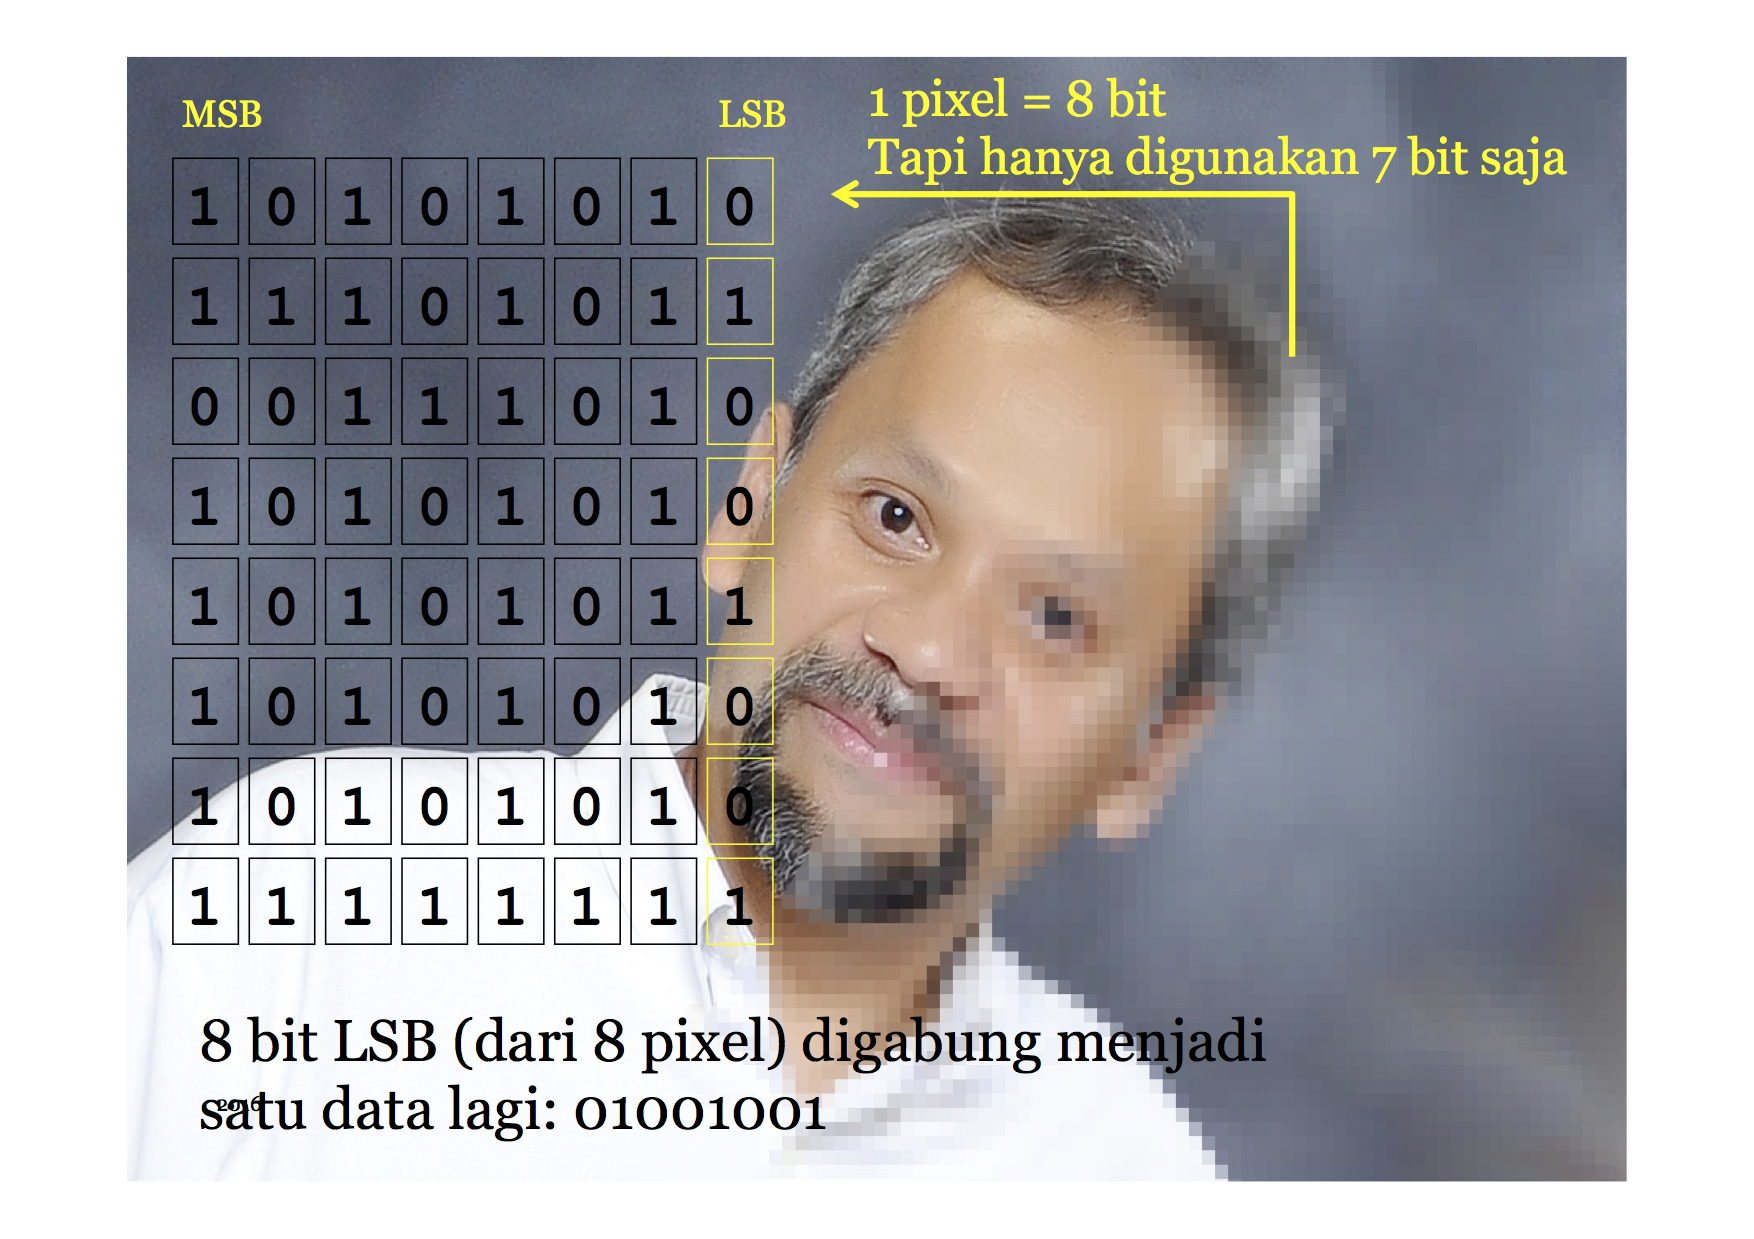
\includegraphics[width=1.0\linewidth]{graphics/BR-watermark.png}}
\caption{Contoh Watermark}
\label{fig:watermark}
\end{figure}

Ada banyak cara untuk menyisipkan informasi ke dalam berkas digital. Sebagai
contoh, kita dapat menyisipkan pesan di dalam gambar (foto) digital seperti
ditampilkan pada Gambar~\ref{fig:watermark}. Cara yang digunakan adalah
dengan menggunakan {\em least significant bit} (LSB) dari data {\em pixel}
gambar. Misalnya, sebuah {\em pixel} (titik) di gambar direpresentasikan oleh
8-bit. Dalam hal ini ada 256 kombinasi (katakanlah skala abu-abu / grey scale).
Maka kita dapat mengorbankan bit yang ke-8 tersebut dan hanya menggunakan 7-bit
saja dalam pewarnaan. Bit ke-8 dapat kita gunakan sebagai bagian dari data.
Jika ada 8 bit yang berurutan kita perlakukan seperti itu, maka akan ada tempat
untuk 8-bit data (1 byte). Jika ini kita teruskan lagi, maka kita dapat
menyimpan beberapa (banyak) bytes di dalam gambar itu.
Data yang kita simpan di dalam berkas (gambar) tersebut dapat berupa
kepemilikan gambar, {\em copyright}, misalnya. 

Tentu saja contoh di atas agak sedikit menyederhanakan permasalahan.
Steganografi yang bagus akan tahan bantingan terhadap proses-proses tertentu.
Sebagai contoh, jika gambar tersebut diubah ukurannya ({\em resize}) maka
informasi yang ditanamkan tersebut akan hilang. Algoritma steganografi yang
bagus akan memiliki kekuatan yang lebih dari itu.


\section{Kriptografi}
Berbeda dengan steganografi, kriptografi tidak menyembunyikan pesan tetapi
mengubah pesan sehingga sulit diperoleh pesan aslinya. Pesan diubah dengan cara
{\bf transposisi} (mengubah letak dari huruf) dan {\bf substitusi} (mengganti
huruf/kata dengan huruf/kata lainnya). Pesan yang sudah diubah terlihat seperti
sampah, tetapi tetap terlihat oleh penyerang atau orang yang tidak berhak.

Proses transposisi dapat dilakukan dengan berbagai cara. Sebagai contoh, kita
dapat menulis pesan menjadi dua baris secara bergantian. Huruf pertama
diletakkan di baris pertama, huruf kedua di baris kedua, huruf ketiga di baris
pertama lagi, huruf keempat di baris kedua lagi, dan seterusnya. Mari kita
ambil contoh kalimat ``selamat datang di kota bandung''. Kalimat ini akan kita
tuliskan secara bergantian. (Dalam contoh ini, spasi kita buang saja.)

\begin{mdframed}
\begin{verbatim}
slmtaagioaadn
eaadtndktbnug
\end{verbatim}
\end{mdframed}

Kalimat yang akan dikirimkan menjadi ``slmtaagioaadneaadtndktbnug''. Kalimat
ini yang kita kirimkan. Dapat dilihat bahwa kalimat yang dikirimkan sudah sulit
dibaca isinya. Di sisi penerima akan dilakukan proses sebaliknya sehingga
didapat kalimat aslinya. Ini adalah salah satu contoh proses transposisi.

Proses substitusi dalam kriptografi dilakukan dengan menukarkan simbol dengan
simbol lain. Sebagai contoh kita dapat menukarkan huruf dengan huruf lain
sesuai dengan sebuah aturan. 

{\bf Caesar cipher} merupakan salah satu contoh kriptografi dengan menggunakan
metoda substitusi. Cara kerjanya adalah sebagai berikut. Urutkan huruf abjad
dari ``A'' sampai ke ``Z''. Di bawahnya kita geser huruf-huruf tersebut
sebanyak tiga lokasi. Hasilnya seperti terlihat di bawah ini. (Penggunaan huruf
besar dan kecil hanya untuk memperjelas saja. Seharusnya kedua baris memiliki
huruf yang sama.)

\begin{mdframed}
\begin{verbatim}
A B C D E F G H I J K L M N O P Q R S T U V W X Y Z
d e f g h i j k l m n o p q r s t u v w x y z a b c
\end{verbatim}
\end{mdframed}

Katakan kita ingin mengirim pesan yang berisi kata ``BUDI''. Yang kita lakukan
adalah mengambil huruf-huruf di bawah masing-masing huruf sebagai penggantinya.
Sebagai contoh, huruf ``B'' akan digantikan dengan ``e', ``U'' digantikan
``x'', ``D'' digantikan ``g'', dan ``I'' digantikan ``l''. Sehingga ``BUDI''
akan menjadi ``EXGL''.

Jumlah pergeseran huruf - apakah 3 atau 7 - dapat ditentukan bersama. Namun ada
yang menarik jika kita gunakan 13 sebagai jumlah pergeseran. Jumlah huruf kita
ada 26, sehingga 13 merupakan angka ``ajaib''. Sebuah pesan dapat kita geser 13
sehingga menjadi tersembunyi dan kalau kita geser 13 lagi (dengan proses yang
sama) akan menghasilkan teks aslinya. Proses ini dikenal dengan istilah {\bf
ROT13} (atau rotate 13)~\footnote{Ada situs www.rot13.com yang dapat kita
gunakan untuk melakukan enkripsi dan dekripsi dengan pergeseran 13 huruf itu.}.

\begin{mdframed}                                                                   
\begin{verbatim} 
FHQNUXNU NAQN ZRAPBON?
\end{verbatim}
\end{mdframed}                                                                   

Cara substitusi seperti yang digunakan oleh {\em Caesar cipher} tersebut
menggunakan satu tabel sehingga sebuah huruf akan disubstitusi oleh huruf yang
sama. Dalam contoh pertama, huruf ``B'' akan disubstitusi dengan huruf ``E''.
Hal ini disebut {\em monoaplhabetic cipher}.

Persandian dengan menggunakan {\em Caesar cipher} ini bertahan cukup lama.
Dapatkah Anda membayangkan cara memecahkan persandian ini? Serangan (attack)
apa yang dapat Anda lakukan? Ternyata Al Kindi menemukan cara untuk memecahkan
{\em Caesar cipher} ini.

Kelemahan dari {\em monoalphabetic cipher} adalah huruf yang sama digantikan
oleh huruf pasangannya dan tetap seperti itu. Serangan yang dilakukan oleh Al
Kindi adalah membuat statistik dari kemunculan huruf. Dalam sebuah bahasa
tertentu, katakan Bahasa Inggris, ada statistik kemunculan setiap huruf. Dalam
Bahasa Inggris, huruf yang paling sering muncul adalah huruf ``A''. Jika hasil
statistik dari teks yang sudah tersandikan huruf yang paling sering muncul
adalah huruf ``J'', maka kita tinggal geser huruf ``J'' tersebut di bawah huruf
``A'' dan sisanya tinggal menyesuaikan. Ternyata tidak susah untuk melakukan
serangan bukan?

\begin{mdframed}[backgroundcolor=blue!20]
\begin{ExerciseList}
   \Exercise[title=Kemunculan huruf]
   \Question{Buat sebuah program yang membuat statistik kemunculan huruf-huruf
   untuk bahasa Indonesia, bahasa Inggris, bahasa Jawa, dan bahasa Sunda.
   Urutkan lima terbesar di setiap bahasa. Catatan: Semakin banyak Anda memberi
   masukan kepada program statistik Anda, semakin akurat hasil statistiknya.}
   \Question{Apakah metoda ini dapat digunakan untuk bahasa-bahasa yang tidak
   menggunakan karakter Roman (seperti bahasa Arab, Cina, India, Thailand, dan
   sejenisnya)?}
\end{ExerciseList}
\end{mdframed}


Dalam sejarah persandian, keberadaan orang yang membuat algoritma sandi ({\em
code maker}) akan berseteru dengan orang yang berusaha untuk memecahkannya
({\em code breaker}). Dalam contoh di atas, Al Kindi menjadi {\em code breaker}
yang memecahkan kode {\em Caesar cipher}.


\subsection{Struktur Sistem Kriptografi}
Secara umum ada tiga komponen utama dari kriptografi, yaitu {\em plain text},
{\em ciphertext}, dan algoritma serta kunci yang digunakan\footnote{Pada
awalnya, kunci melekat dengan algoritma. Namun kemudian, kunci dipisahkan dari
algoritma. Kekuatan dari sebuah sistem kriptografi bergantung kepada
kerahasiaan dari kuncinya, bukan dari kerahasiaan algoritmanya.}.
\begin{itemize}
  \item {\em Plain text} adalah data (teks, pesan, {\em message}) asli yang
  belum diproses. Meskipun disebut plain text, sesungguhnya data asli tidak
  harus berupa teks (ASCII). Plain text dapat juga berupa berkas biner.
  \item {\em Ciphertext} adalah data yang dihasilkan dari proses enkripsi.
     {\em Ciphertext} dapat berbentuk berkas biner atau ASCII. Perlu diasumsikan
  bahwa penyerang kemungkinan dapat mengakses ciphered text.
  \item Algoritma dan kunci merupakan {\em black box} yang memproses plain text
  menjadi ciphered text. Algoritma diasumsikan diketahui oleh penyerang,
  tetapi kunci tidak diketahui.
\end{itemize}

Hubungan antara ketiga komponen tersebut dapat dirumuskan sebagai berikut.
{\em Ciphertext} $c$ merupakan hasil operasi enkripsi ({\em encryption}) $E$ 
dengan kunci $k$ terhadap pesan $m$. {\em Ciphertext} ini yang nanti dikirimkan
kepada pihak yang dituju.

\begin{equation}
   c = E_k(m)
\end{equation}

Di sisi sebaliknya, yaitu di sisi penerima, pesan ({\em plain text}) $m$
diperoleh dari hasil proses dekripsi ({\em decryption}) $D$ dengan kunci $k$
terhadap {\em ciphertext} $c$.

\begin{equation}
   m = D_k(c)
\end{equation}

Jika kita menggunakan algoritma kriptografi kunci privat, yang akan dibahas
kemudian, kunci ($k$) yang sama digunakan untuk proses enkripsi dan dekripsi.
Untuk algoritma kriptografi yang berbasis kunci public, kunci yang digunakan
untuk proses enkripsi dan dekripsi berbeda.


\subsection{Kriptografi Kunci Privat}
Kriptografi kunci privat adalah jenis kriptografi yang paling banyak dikenal.
Pada sistem kriptografi ini, ada satu kunci yang digunakan untuk mengunci dan
membuka. Itulah sebabnya sistem ini dikenal juga dengan istilah kriptografi
{\bf simetrik}. Kunci yang digunakan harus dirahasiakan sehingga kriptografi
ini disebut kriptografi kunci privat.

Ada banyak algoritma yang mengimplementasikan kriptografi kunci privat, antara
lain DES, Blowfish, dan AES. (Penjelasan rinci mengenai algoritma-algoritma ini
akan dibahas secara terpisah.) Algoritma-algoritma ini umumnya sangat cepat
dalam operasinya.

Salah satu kesulitan dari pengoperasian sistem kriptografi kunci privat adalah
dalam hal distribusi kunci ({\em key distribution}). Sebagai contoh, jika {\em
Alice} ingin mengirim pesan kepada {\em Bob}, maka mereka berdua memiliki
sebuah kunci yang sama. Jika {\em Alice} ingin mengirim pesan ke orang lain,
katakan {\em Charlie}, maka mereka berdua memiliki kunci sendiri ({\em
Alice-Charlie}) yang berbeda dengan kunci {\em Alice-Bob}. Demikian pula jika
{\em Bob} dan {\em Charlie} ingin berkomunikasi maka mereka memiliki kunci
sendiri ({\em Bob-Charlie}). Jika kita teruskan dengan pihak-pihak lain, maka
jumlah kunci yang dibutuhkan akan meledak secara eksponensial sesuai dengan
penambahan jumlah pengguna ($n$).

\begin{equation}
   numkeys = \frac{(n) (n-1)}{2}
\end{equation}

Untuk jumlah pengguna yang sedikit, misal puluhan orang, maka jumlah kunci yang
beredar tidak terlalu banyak. Begitu jumlah pengguna sangat banyak, maka jumlah
kunci menjadi sangat besar seperti dapat dilihat pada
tabel~\ref{tbl:jumlahkunci}. Bayangkan jumlah pengguna internet di dunia ini.
Berapa banyak kunci yang harus dipersiapkan jika semuanya akan saling
berkomunikasi satu dengan lainnya?

\begin{table}
   \centering
   \caption{Jumlah Kunci}
   \label{tbl:jumlahkunci}
\begin{tabular}{ r r }
   $n$ & Jumlah kunci \\
   \hline
  10 & 45 \\
  100 & 4.950 \\
  1000 & 499.500 \\
  10.000 & 49.995.000 \\
  100.000 & 4.999.950.000 \\
\end{tabular}
\end{table}

Meskipun ada masalah distribusi kunci, sistem kriptografi kunci privat ini yang
paling baik kinerjanya (performance) sehingga dia sangat dibutuhkan.


\subsection{Kriptografi Kunci Publik}
Pada sistem kriptografi kunci publik, ada dua kunci yang akan digunakan. Setiap
pelaku akan memiliki sepasang kunci ({\bf kunci publik} dan {\bf kunci privat})
yang saling berhubungan. Jika sebuah pesan dikunci dengan kunci publik, maka
dia hanya dapat dibuka oleh kunci privat pasangannya. Demikian pula jika sebuah
pesan dikunci oleh kunci privat, maka dia hanya dapat dibuka oleh kunci publik
pasangannya. (Jangan bingung. Baca berulang kali. Nanti akan dijelaskan dengan
cara lain lagi.)

Sistem ini sering juga disebut {\bf kriptografi asimetrik}, karena kunci yang
dipakai untuk mengunci berbeda dengan kunci untuk membuka. Asimetrik.

Sesuai dengan namanya, kunci publik boleh diketahui oleh umum dan disimpan di
tempat publik. Sementara itu, kunci privat hanya boleh diakses oleh pemiliknya.
Selama-lamanya kunci privat ini tidak boleh terbuka. Jika kunci privat ini
tercuri, maka identitas kita juga tercuri.

Mari kembali kita ambil contoh komunikasi antara {\em Alice} dan {\em Bob}.
Masing-masing pelaku memiliki sepasang kunci. {\em Alice} memiliki kunci publik
$KA_{pub}$ dan kunci privat $KA_{priv}$. Demikian pula {\em Bob} memiliki kunci
publik $KB_{pub}$ dan kunci privat $KB_{priv}$. Jika {\em Alice} ingin
mengirimkan pesan $m$ kepada {\em Bob}, maka {\em ciphertext} $c$ merupakan
hasil enkripsi dengan menggunakan kunci publik {\em Bob}.

\begin{equation}
   c = E_{KB_{pub}}(m)
\end{equation}

Di sisi penerima, {\em Bob}, akan menerima cipertext $c$. Untuk
mengembalikannya ke pesan semula, dilakukan proses dekripsi ($D$) dengan kunci
privatnya sebagai berikut. Perlu diingat bahwa hanya {\em Bob} yang dapat
melakukan hal ini karena hanya dia yang memiliki kunci privatnya. {\em Alice}
sebagai pengirim pun sudah tidak dapat membuka kembali pesan yang dia kirimkan.

\begin{equation}
   m = D_{KB_{priv}}(c)
\end{equation}

Yang menarik dari proses ini adalah untuk mengirimkan pesan bersandi ke {\em
Bob}, sang pengirim ({\em Alice}) hanya perlu mencari kunci publik {\em Bob}.
Dia tidak perlu bertukar kunci sebelumnya. Masalah {\em key distribution}
terpecahkan dengan cara ini.

Jumlah kunci yang beredar di sistem juga tidak meledak sebagai mana terjadi
pada kriptografi kunci privat. Jika jumlah pengguna adalah $n$, maka jumlah
kunci adalah:

\begin{equation}
   numkeys = 2n
\end{equation}

Beberapa contoh algoritma kriptografi kunci publik yang terkenal antara lain
RSA dan Elliptic Curve Cryptosystem (ECC). Sayangnya algoritma-algoritma ini
memiliki komputasi yang cukup tinggi. (Akan dibahas kemudian.) Akibatnya,
algoritma kriptografi kunci publik kurang disukai atau digunakan secukupnya
saja.

\chapter{PGP / Gnu Privacy Guard}
Pretty Good Privacy (PGP) pada awalnya adalah aplikasi yang dapat digunakan
pengguna untuk menggunakan kriptografi di berbagai aplikasi dengan lebih mudah.
Pengembangan selanjutnya PGP menjadi bagian dari {\em public key
infrastructure}.

\section{Sejarah}
[... more to be written ...]

Gnu Privacy Guard (GPG) merupakan implementasi dari PGP yang bersifat terbuka.
(Catatan: Singkatan dari GPG ini merupakan guyonan terhadap PGP.) Bab ini akan
membahas lebih banyak tentang GGP, meskipun konsep yang sama dapat juga
diterapkan pada PGP jika Anda menggunakan produk PGP yang komersial.

Dalam buku ini, kita akan menggunakan GPG versi {\em command line interface},
yaitu dengan mengetikkan perintah ``gpg'' di program terminal atau CMD.exe.
Ada banyak program {\em GUI} dari GPG ini. Silahkan gunakan manual terkait
dengan program-program tersebut. Prinsipnya masih tetap sama.

\section{Menggunakan Gnu Privacy Guard, gpg}
Awal dari penggunakan GPG adalah membuat pasangan kunci publik dan privat. Hal
ini dapat dilakukan dengan menggunakan perintah berikut.

\begin{verbatim}
gpg --key-gen
\end{verbatim}

Perintah di atas akan menanyakan beberapa hal, seperti jenis algoritma yang
digunakan (pilih RSA dan RSA), panjang kuncinya (pilih 2048), dan alamat email
yang akan digunakan untuk kunci tersebut. Dalam contoh buku ini saya akan
menggunakan alamat email ``rahard2017@gmail.com''. Gunakan alamat email Anda
sebagai penggantinya/

\begin{verbatim}
$ gpg --gen-key
gpg (GnuPG/MacGPG2) 2.0.30; Copyright (C) 2015 Free Software Foundation, Inc.
This is free software: you are free to change and redistribute it.
There is NO WARRANTY, to the extent permitted by law.

Please select what kind of key you want:
   (1) RSA and RSA (default)
   (2) DSA and Elgamal
   (3) DSA (sign only)
   (4) RSA (sign only)
Your selection? 1
RSA keys may be between 1024 and 4096 bits long.
What keysize do you want? (2048)
Requested keysize is 2048 bits
Please specify how long the key should be valid.
         0 = key does not expire
      <n>  = key expires in n days
      <n>w = key expires in n weeks
      <n>m = key expires in n months
      <n>y = key expires in n years
      Key is valid for? (0) 3m
Key expires at Wed May 31 10:30:37 2017 WIB
Is this correct? (y/N) y

GnuPG needs to construct a user ID to identify your key.

Real name: Budi Rahardjo
Email address: rahard2017b@gmail.com
Comment:
You selected this USER-ID:
    "Budi Rahardjo <rahard2017@gmail.com>"

Change (N)ame, (C)omment, (E)mail or (O)kay/(Q)uit?
\end{verbatim}

Setelah proses {\em key generation} selesai, kunci publik dapat diekspor dengan
menggunakan perintah  berikut. Gantikan ``rahard2017@gmail.com'' dengan alamat
email Anda.

\begin{verbatim}
gpg --export --armor rahard2017@gmail.com > kunci-public.asc
\end{verbatim}

Akan dihasilkan berkas ``kunci-public.asc''. Tanpa perintah {\em redirect
output} yang menggunakan ``>'' itu, hasilnya hanya akan ditampilkan di layar
saja. Tentu saja Anda dapat menggunakan nama berkas lainnya.
Berikut ini adalah contoh beberapa baris pertama dari berkas ASCII hasil ekspor
kunci tersebut. (Tampilan bisa panjang sekali, bergantung dari panjang kunci
yang digunakan.)

\begin{verbatim}
-----BEGIN PGP PUBLIC KEY BLOCK-----
Comment: GPGTools - https://gpgtools.org

mQENBFiiijUBCAD3ZIxjUQyDtcGTmHs2iU+2aS+MMp2w+codVRrqLfVI+V8S+TmP
WGe2Gu4pTLovGzZ2NGWvKACZ0A+BL97e9K6QN6+UIYRArFdxfojQ4lbwH/WO1YSn
J6BsCE1IfX8niRiskdibBhZZcrUCcDa/tgvgXTymoAeZEcMwR48hEOUWuOGoCE2g
TA/kD9yCyorFUKEsbyKJMKPtlMJGICUwtggDdXT5arCCafpydLGxok+w4TJjADeX
jeTxDgYSNjCNar9wRhtnG+G/Irbfctj77/9Ppz8j8Dp1NkAwx5P+9AJRNNkwU88c
7FSEz0cpAzgC4VyaL/iX85G8wr6z5kaWNV3FABEBAAG0JEJ1ZGkgUmFoYXJkam8g
PHJhaGFyZDIwMTdAZ21haWwuY29tPokBPQQTAQoAJwUCWKKKNQIbAwUJABuvgAUL
...
\end{verbatim}

Kunci publik ini yang akan didistribusikan secara publik, misal disimpan di
blog Anda. Kunci ini juga dapat disimpan di {\em key server}.

Untuk melihat informasi mengenai kunci Anda, dapat digunakan perintah berikut:

\begin{verbatim}
gpg --fingerprint rahard2017

pub   2048R/EB6CEB46 2017-02-14 [expires: 2017-03-07]
      Key fingerprint = 810B 2149 3366 E699 F95E  9E49 07E1 BDC5 EB6C EB46
uid       [ultimate] Budi Rahardjo <rahard2017@gmail.com>
sub   2048R/C2E83C60 2017-02-14 [expires: 2017-03-07]
\end{verbatim}

Perhatikan bahwa kunci publik yang ini memiliki ID ``EB6CEB46''. ID ini dapat
digunakan untuk bertukar kunci, atau untuk melakukan proses-proses lainnya.
Sebagai contoh, kita dapat mengirimkan kunci ini ke server agar dapat dilihat
atau dicari oleh orang lain. Keyserver yang akan kita gunakan dalam contoh ini
adalah pgp.mit.edu.

\begin{verbatim}
gpg --keyserver pgp.mit.edu --send-keys EB6CEB46
\end{verbatim}

Pengirimkan kunci dapat juga dilakukan dengan menggunakan web dari situs PGP
MIT tersebut sebagaimana dicontohkan dalam gambar berikut. Masukkan teks ASCII
kunci Anda ke kolom kunci dan upload.

\begin{figure}[ht]
\fbox{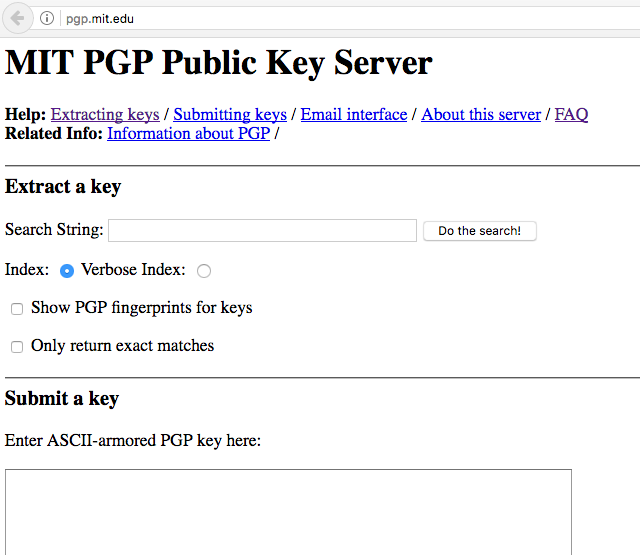
\includegraphics[width=1.0\linewidth]{graphics/pgp-mit.png}}
\caption{Key server pgp.mit.edu}
\label{fig:pgp-mit}
\end{figure}


\begin{mdframed}[backgroundcolor=blue!20] 
\begin{ExerciseList}
   \Exercise[title=Membuat Kunci]
   \Question{Buat pasangan kunci publik dan kunci privat Anda. Gunakan parameter
   default saja (RSA dan RSA). Asosisasikan dia dengan alamat email Anda.} 
   \Question{Unggah kunci publik Anda ke salah satu keyserver yang tersedia 
   (misal pgp.mit.edu atau keyserver.cert.or.id)} 
   \Question{Beritahukan teman-teman Anda tentang kunci Anda tersebut. Minta
   mereka untuk ikut menandatangani kunci publik Anda tersebut.}
\end{ExerciseList}

\end{mdframed}

\subsection{Enkrip Untuk Sebuah Alamat Email}
Salah satu fungsi dari PGP/GPG adakan mengirim pesan secara rahasia. Pesan
tersebut dienkrip dengan menggunakan kunci publik (alamat email) tujuan.
Sebagai contoh, kita akan mencoba mengirimkan pesan rahasia ke
rahard2017@gmail.com.

Langkah pertama tentunya kita harus mendapatkan kunci publik dari akun email
rahard2017 tersebut. Cari di salah satu keyserver, unduh, dan masukkan ke
gantungan kunci kita.

\begin{verbatim}
gpg --keyserver hkp://pgp.mit.edu --search-keys rahard2017
\end{verbatim}

Dalam contoh ini, kita akan menggunakan berkas ``dokumen.txt'' yang berisi
pesan dalam bentuk {\em plain text}. Tentu saja PGP/GPG tidak membatasi jenis
pesan (berkas). Dalam contoh ini saja kita akan menggunakan berkas teks yang
berisi teks ASCII. Secara umum berkas biner (MS Word, lagu MP3, film MP4, dan
seterusnya) dapat juga diproses. Isi berkas dokumen.txt tersebut adalah sebagai
berikut.

\begin{mdframed}[backgroundcolor=blue!20] 
\begin{verbatim}
Ini adalah dokumen untuk percobaan menggunakan PGP/GPG.
Untuk tanda tangan, isinya tidak harus disembunyikan.
Selamat mencoba.
\end{verbatim}
\end{mdframed}

Perintah untuk mengenkripsi dengan menggunakan kunci publik tujuan
(rahard2017@gmail.com) adalah seperti dicontohkan di bawah ini. Perintah
tersebut akan menghasilkan berkas ``dokumen.pgp''.

\begin{verbatim}
gpg --output dokumen.pgp --encrypt --recipient rahard2017@gmail.com dokumen.txt
\end{verbatim}

Berkas ``dokumen.pgp'' yang dihasilkan dari proses enkripsi di atas berupa
berkas biner. Jika kita ingin menghasilkan berkas dalam bentuk ASCII, maka
gunakan opsi ``-armor'' (-a) seperti perintah di bawah ini.

\begin{verbatim}
gpg -a --output dokumen.pgp --encrypt --recipient rahard2017@gmail.com dokumen.txt
\end{verbatim}

Jika kita lihat berkas ``dokumen.pgp'', isinya adalah seperti berikut.

\begin{mdframed}
\begin{verbatim}
-----BEGIN PGP MESSAGE-----
Comment: GPGTools - https://gpgtools.org

hQEMAy/vbaXC6DxgAQf/Zjk74t1FXTT3abmJUz/w5Z8iHIIEWZlvMmBdMS7w/2U8
L2NvrvG6GOrsduLTIrybCIAQ0GPU9Nq+YOMYJaY3BhiqkCSyYhHYRk0406OS3GCA
ONnhiqKiVLJIyfNWdDBtB4k7s8pfM5ngxgeZ6/gH5TDspHrhjrLS65Stn7sr+Nlf
TSuG9p21vr19yL13KBkd2rI5WBnL68/3bRJnKt0JL1PLeMvQ0eZIiRXcmropPXIs
rltFRflpdp0H0LJn2/xQ5rXr13QRRjzo3SL4i/eYxPlEmpD164aicI8LC+qKgYcc
FShUuTxwxtu7tPYpqEH17jTTd29wZdrXDFHp5TGLTdKtAeMKeGupxvicOaNMY46J
S3LBC9fU2bywwmvM77cCr97DOP1rA6WXR2xluRvLhms83lNMcpSDuZCPpb8rxKmu
Xk2WFThfV5rq0I1kyP2Kc1g+0cgnJkAzFXe5MQRIOpJ/MRwrekAo3Dvp3TefwMYu
R3LYwCi8VstPpnH9rcFyoyxsqMqLTPtUnheISNUmVERtLm3rALtHjf2vyvkR/2JF
Vmu79aqbbFJPJZ0gNmk=
=D+3L
-----END PGP MESSAGE-----
\end{verbatim}
\end{mdframed}

Berkas ``dokumen.pgp'' tersebut dapat kita kirimkan (misal melalui email) ke
rahard2017@gmail.com. Di sisi penerima (rahard2017), berkas tersebut dapat dia
buka dengan menggunakan kunci privatnya. Ketika menggunakan kunci privat,
biasanya pengguna ditanyakan {\em passphrase} untuk mengakses (membuka) kunci
privat tersebut karena biasanya kunci privat dilindungi dengan {\em passphrase}
tersebut.

\begin{mdframed}
\begin{verbatim}
gpg --decrypt dokumen.pgp

You need a passphrase to unlock the secret key for
user: "Budi Rahardjo <rahard2017@gmail.com>"
2048-bit RSA key, ID C2E83C60, created 2017-02-14 (main key ID EB6CEB46)

gpg: encrypted with 2048-bit RSA key, ID C2E83C60, created 2017-02-14
      "Budi Rahardjo <rahard2017@gmail.com>"
Ini adalah dokumen untuk percobaan menggunakan PGP/GPG.
Untuk tanda tangan, isinya tidak harus disembunyikan.
Selamat mencoba.
\end{verbatim}
\end{mdframed}

Seperti dilihat pada contoh di atas, teks aslinya ditampilkan di layar. Jika
kita ingin menyimpannya ke dalam sebuah berkas, maka dapat kita gunakan opsi
``--output namaberkas'' ketika menjalankan perintah gpg tersebut di atas.

Perlu diingat kembali bahwa hanya orang yang memiliki kunci privat, yaitu
rahard2017@gmail.com, yang dapat membuka berkas tersebut. Jika berkas tersebut
dicoba untuk dibuka dengan kunci lain, maka dia tidak dapat menghasilkan isi
yang sama.

\subsection{Tanda Tangan Dokumen}
Salah satu manfaat penggunaan PGP/GPG adalah tanda tangan digital (sign). Dalam
contoh berikut ini kita akan mendatangani berkas ``dokumen.txt''. (Kita dalam
contoh ini adalah ``rahard2017@gmail.com''.)

\begin{verbatim}
gpg -u rahard2017@gmail.com --output dokumen.sig --sign dokumen.txt

You need a passphrase to unlock the secret key for
user: "Budi Rahardjo <rahard2017@gmail.com>"
2048-bit RSA key, ID EB6CEB46, created 2017-02-14
\end{verbatim}

Seperti sebelumnya, berkas yang dihasilkan (dokumen.sig) dalam format biner.
Untuk menghasilkan berkas ASCII, dapat digunakan ``-a''.

\begin{verbatim}
gpg -a -u rahard2017@gmail.com --output dokumen.sig --sign dokumen.txt
\end{verbatim}

Isi berkas ``dokumen.sig'' yang sudah di-armor-kan seperti ini. Sebagai
catatan, isi dokumen dan tanda tangan tercampur dan ter-armor-kan. Kerugian
cara ini adalah isi dari dokumen tidak dapat terlihat secara langsung.

\begin{verbatim}
-----BEGIN PGP MESSAGE-----
Comment: GPGTools - https://gpgtools.org

owGbwMvMwMXI/nDv0dc5r90Y10xI4k7Jzy7NTc3TK6koidipudUzL1MhMSUxJzFD
ASqjUJpXUpqtUJBalJyflJiYpwAUS08vzUvMBrID3AP03QPc9bhCwYpKEvNSEkFk
emKejkJmcWZeJZCbmZKYrZCRWFRarJCSWZyam1SaV5kJ1K3HFZyak5ibWAIyEmS4
HlcnowwLAyMXAxsrE8g1DFycAjDXcoix//d7pfhQ+pbBxM4ilx/pi054OOkFsfS2
TDDSVY/Zec58cp/zm9TgDczKn+71Kkqvs/4fNNvRuUr208VdwowLPTliFpR+O2/L
0cR/KDTuie6h9Xlq3bXTSg6kpeoxblZ323ra4jDfvvs/9RjeSByS0cp4+T/c81B6
YUepNtO0hLjZZeGxR63yNqxbu7ZX9djt4p6a7/JTbJKepvo3XItlO8x0xVDt3LIv
oRc/tc7667WqskaC95zr1E6xREHL5eEKGnkByy7arEnL0Ge++bNd4ET4NOV3FYqP
L875kT8v8PeVPdqr+SrENG7YNL6+PWXOvNUR6ruMVdSOhzEoeyn4P2EWX6J1dVL/
n1dzXzdrAgA=
=VRfS
-----END PGP MESSAGE-----
\end{verbatim}

Ada cara untuk memisahkan isi (teks) dan tanda tangannya. Perintah yang
digunakan adalah ``--clearsign''.
\begin{verbatim}
gpg -u rahard2017@gmail.com --output dokumen.sig --clearsign dokumen.txt
\end{verbatim}

Hasilnya adalah sebuah berkas yang isinya adalah sebagai berikut. Perhatikan
bahwa isi dan tanda tangan terpisah, meskipun masih dalam sebuah berkas.

\begin{mdframed}[backgroundcolor=red!20]
\begin{verbatim}
-----BEGIN PGP SIGNED MESSAGE-----
Hash: SHA512

Ini adalah dokumen untuk percobaan menggunakan PGP/GPG.
Untuk tanda tangan, isinya tidak harus disembunyikan.
Selamat mencoba.
-----BEGIN PGP SIGNATURE-----
Comment: GPGTools - https://gpgtools.org

iQEcBAEBCgAGBQJYuSthAAoJEAfhvcXrbOtG1pkIALaFxIxKObM7p/ZTMpzNCIHN
GpyR9Q6QQEi+9+0loHdw1TqMEskJ3HxWOnegupMueiIpO0IaEd8qCraLSfRF3G1f
gBxl837rXnTjDIYABN9T6f5GrZHyeWXEhwDRDuLWsb9v85pNd/RUbQ8L7N/s4SUl
NgyPbHKhal+ob047mHE1zF9lvpuRfhWM3ztr8OJN6MWTgb+NYpc0b9YuyqSRiDZ0
y3fvY3iRexMjLI2dxhXOTWG4IM5ouwbFtheJML1Lssh/pn1KZwicnWGAouWhQTOY
hGR8zSoy4oeS/hlUmdAu3bse73pcWeybCtYLwvXSBvg7W67sCOERmIfZxXxtq08=
=/uVR
-----END PGP SIGNATURE-----
\end{verbatim}
\end{mdframed}

Untuk melakukan verifikasi apakah dokumen tersebut terjamin integritasnya
(isinya tidak berubah dan yang menandatangani benar), gunakan perintah
``verify''.

\begin{mdframed}
\begin{verbatim}
gpg --verify dokumen.sig
\end{verbatim}
\end{mdframed}


Seringkali ada kebutuhan untuk memisahkan berkas dari tanda tangan dan
dokumennya. Sebagai contoh, jika dokumen yang ingin kita tandatangani adalah berkas
biner (dokumen {\em word processor}, audio, video, dan sejenisnya), maka tanda
tangan dan dokumennya harus dipisah.

\begin{verbatim}
gpg -u rahard2017@gmail.com --output dokumen.sig --detach-sig dokumen.txt
\end{verbatim}

Untuk melakukan verifikasi bahwa dokumen tersebut benar (isinya benar dan yang
menandatangani benar juga) jika dokumennya dipisah adalah sebagai berikut.

\begin{mdframed}
\begin{verbatim}
gpg --verify dokumen.sig dokumen.txt
\end{verbatim}
\end{mdframed}

\begin{mdframed}[backgroundcolor=blue!20]
\begin{ExerciseList}
   \Exercise[title=Verifikasi]
   \Question{Menurut Anda, apakah tanda tangan (signature) akan tetap sama
   untuk setiap orang meskipun dokumen yang ditandatangani berbeda-beda?
   Ataukah untuk dokumen yang berbeda, tanda tangan digital dari dokumen 
   tersebut akan berbeda?}
   \Question{Verifikasi dokumen dengan data yang benar. Maksudnya jangan ubah
   berkas ``dokumen.sig'' dan ``dokumen.txt''.}
   \Question{Verifikasi dokumen dengan data yang sudah tercemar. Edit berkas
   dokumen.txt sehingga berbeda dengan aslinya. Coba verifikasi. Tunjukkan
   bahwa proses verifikasi gagal.}
\end{ExerciseList}
\end{mdframed}

\section{Tools}
Perintah-perintah dalam contoh pada bagian sebelumnya dilakukan dengan
menggunakan {\em command line}. Ada beberapa {\em tools} (biasanya memiliki
{\em graphical user interface}) yang dapat membantu untuk mempermudah operasi.
{\em Tools} yang tersedia bergantung kepada sistem operasi yang Anda gunakan. 


\section{Web of Trust}
Keamanan dari PGP/GPG ini berbasis {\em web of trust}. Bagaimana kita dapat
mempercayai bahwa kunci publik tersebut milik dari ``Budi Rahardjo'' dengan
alamat email tersebut (rahard2017@gmail.com)? Boleh jadi ada seseorang yang
dengan sengaja memalsukan identitas tersebut. 

Proses verifikasi dilakukan oleh orang lain dengan menandatangani kunci
tersebut dan kemudian data tersebut - kunci yang sudah ditandatagani - diunggah
kembali ke keyserver. 


\bibliography{referensi}

%\bibliographystyle{plainnat}
%\bibliographystyle{alpha}
\bibliographystyle{plain}

\end{document}
